\documentclass{memoir}
\usepackage[utf8]{inputenc}
\usepackage[usenames,dvipsnames,svgnames,table]{xcolor}
\usepackage[marginparwidth=28mm]{geometry}
\usepackage[pdftex]{graphicx}
\usepackage{tikz}

\usepackage{filecontents}
\usepackage[T1]{fontenc}
\usepackage[UKenglish]{babel}
\usepackage{newpxtext,newpxmath}
\usepackage[babel=true]{csquotes}
\usepackage[round]{natbib}
\usepackage[colorinlistoftodos]{todonotes}
\usepackage{comment}
\usetikzlibrary{arrows,automata}
\usepackage{ccaption}
\usepackage{url}
\usepackage{flafter}
\usepackage{pgfplots}
\begin{document}

\newcommand*{\xMin}{-6}%
\newcommand*{\xMax}{6}%
\newcommand*{\yMin}{-6}%
\newcommand*{\yMax}{6}%


\newcommand{\epuck}[3][0] % [angle]{x}{y} avec angle optionel
{
	\draw [very thick, fill=white] (#2,#3) circle [radius=0.5];
	\draw [very thick, rotate around={#1:(#2,#3)}] (#2-0.25,#3-0.433) -- (#2,#3+0.45) -- (#2+0.25,#3-0.433);
}

\newcommand{\epuckred}[3][0] % [angle]{x}{y} avec angle optionel
{
	\draw [very thick, fill=orange] (#2,#3) circle [radius=0.5];
	\draw [very thick, rotate around={#1:(#2,#3)}] (#2-0.25,#3-0.433) -- (#2,#3+0.45) -- (#2+0.25,#3-0.433);
}

\newcommand{\epuckblue}[3][0] % [angle]{x}{y} avec angle optionel
{
	\draw [very thick, fill=RoyalBlue] (#2,#3) circle [radius=0.5];
	\draw [very thick, rotate around={#1:(#2,#3)}] (#2-0.25,#3-0.433) -- (#2,#3+0.45) -- (#2+0.25,#3-0.433);
}

\newcommand{\epuckop}[4][0] % [angle]{x}{y} avec angle optionel
{
	\draw [very thick, fill=white, opacity=#4] (#2,#3) circle [radius=0.5];
	\draw [very thick, , opacity=#4, rotate around={#1:(#2,#3)}] (#2-0.25,#3-0.433) -- (#2,#3+0.45) -- (#2+0.25,#3-0.433);
}

\newcommand{\human}[3][0] % [angle]{x}{y}
{
	\draw [very thick, fill=white, rotate around={#1:(#2,#3)}] (#2-1,#3+0.5) ellipse (0.25cm and 0.5cm);
	\draw [very thick, fill=white, rotate around={#1:(#2,#3)}] (#2+1,#3+0.5) ellipse (0.25cm and 0.5cm);
	\draw [very thick, fill=white, rotate around={#1:(#2,#3)}] (#2,#3) ellipse (1.5cm and 0.75cm);
	\draw [thick, fill=white, rotate around={#1:(#2,#3)}] (#2-0.05,#3+1) -- (#2,#3+1.1) -- (#2+0.05,#3+1);
	\draw [very thick, fill=white, rotate around={#1:(#2,#3)}] (#2,#3+0.5) circle [radius=0.5cm];
}


\chapter{Acknowledgements}
	
	\begin{comment}
		Faire un chemin présentant diverses zones dangereuses. Chaque zone dangereuse contient des problèmes que j'ai rencontrés. La personne qui m'a aidé à la résoudre est affichée sur le chemin à l'endroit où il est dévié.
		Ajouter Céline.
	\end{comment}
	I thank...
	\vfill
	\begin{figure}[!htp]
		\begin{tikzpicture}
		
		\draw[white] (-9.3,0) -- (7,0);
		
		\foreach \i in {0,-1,...,-15} {
			\begin{scope}[rotate around={\i*20:(3,0)}]
				\epuckop{-7.5-\i/1.5}{0}{(15+\i)/15}
			\end{scope}
		}
	\end{tikzpicture}
\end{figure}

		
	
	\begin{figure}[!htp]
		\centering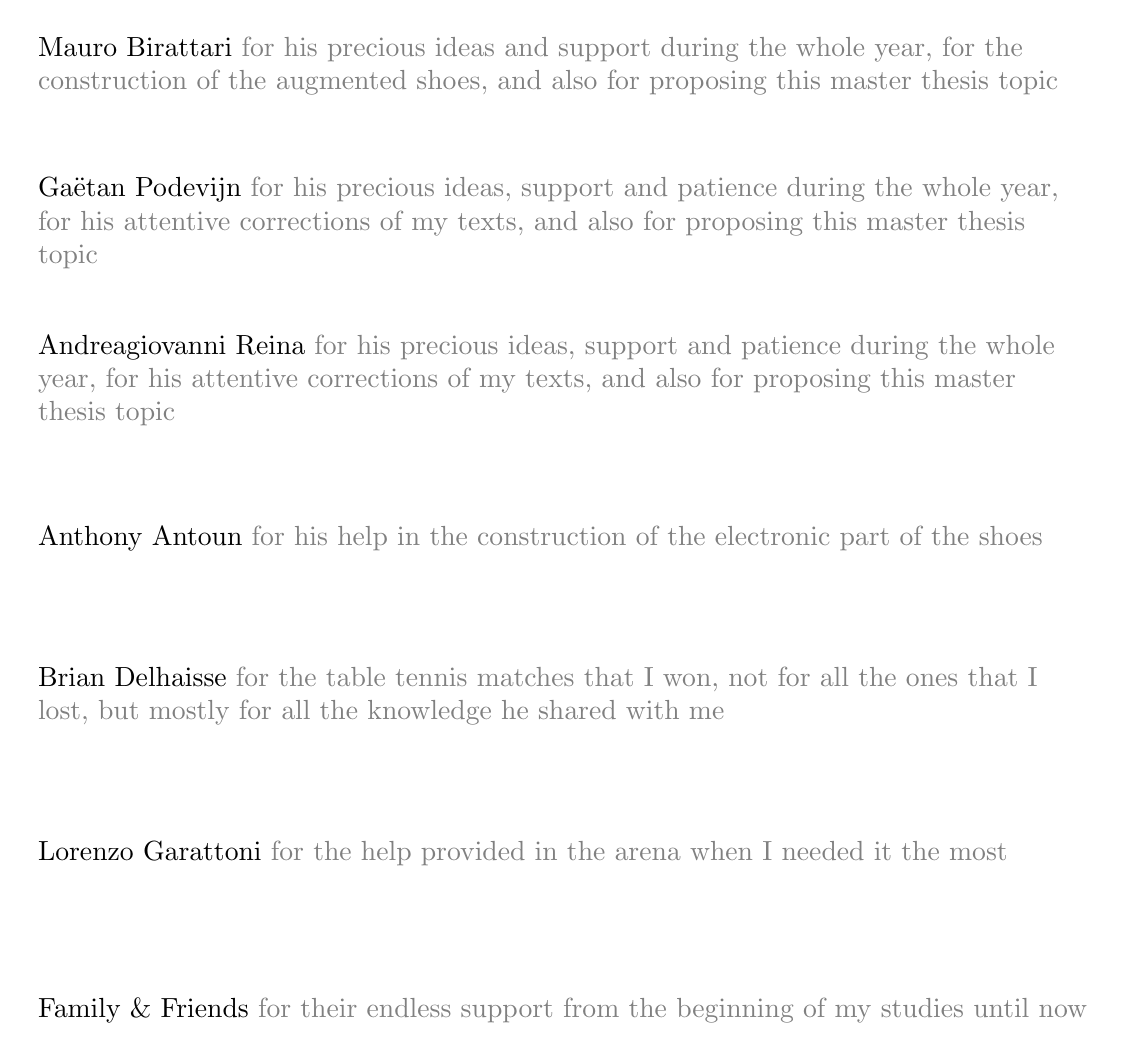
\begin{tikzpicture}
		%Mauro, Gaëtan, Giovanni, Anthony, Lorenzo, Brian, Family and friends.
		\epuck{-7.5}{12}
		\epuck{-7.5}{10}
		\epuck{-7.5}{8}
		\epuck{-7.5}{6}
		\epuck{-7.5}{4}
		\epuck{-7.5}{2}
		%\epuck{-7.5}{0}
		
		\foreach \i in {0,20,...,180} {
			\begin{scope}[rotate around={\i:(0,0)}]
				\epuckop{-7.5}{0}{(180-\i)/180}
			\end{scope}
		}
		
		\draw (-6,12) node[anchor=west, text width=13cm] {Mauro Birattari \color{Gray} for his precious ideas and support during the whole year, for the construction of the augmented shoes, and also for proposing this master thesis topic};
		\draw (-6,10) node[anchor=west, text width=13cm] {Gaëtan Podevijn \color{Gray} for his precious ideas, support and patience during the whole year, for his attentive corrections of my texts, and also for proposing this master thesis topic};
		\draw (-6,8) node[anchor=west, text width=13cm] {Andreagiovanni Reina \color{Gray} for his precious ideas, support and patience during the whole year, for his attentive corrections of my texts, and also for proposing this master thesis topic};
		\draw (-6,6) node[anchor=west] {Anthony Antoun \color{Gray} for his help in the construction of the electronic part of the shoes};
		\draw (-6,4) node[anchor=west, text width=13cm] {Brian Delhaisse \color{Gray} for the table tennis matches that I won, not for all the ones that I lost, but mostly for all the knowledge he shared with me};
		\draw (-6,2) node[anchor=west] {Lorenzo Garattoni \color{Gray} for the help provided in the arena when I needed it the most};
		\draw (-6,0) node[anchor=west] {Family \& Friends \color{Gray} for their endless support from the beginning of my studies until now};
		
		\end{tikzpicture}
	\end{figure}


\begin{figure}\centering
\begin{tikzpicture}

	\clip (-7,-3.1) rectangle (6.1, 4.2);

	\foreach \i in {\xMin,...,\xMax} {
        \draw [very thin,LightGray] (\i,\yMin) -- (\i,\yMax)  node [below] at (\i,\yMin) {$\i$};
    }
    \foreach \i in {\yMin,...,\yMax} {
        \draw [very thin,LightGray] (\xMin,\i) -- (\xMax,\i) node [left] at (\xMin,\i) {$\i$};
    }

	\draw [dashed, fill=red] (3,0) circle [radius=3];
	\draw (3,0) node[scale=5]{!};
	
	\draw[red, fill] (-2.9,0.65) rectangle (-4.1,1.35);
	\draw[LimeGreen, fill] (-2.9,-0.65) rectangle (-4.1,-1.35);
	\draw[BurlyWood, fill] (-3,0.75) rectangle (-4,1.25);
	\draw[BurlyWood, fill] (-3,-0.75) rectangle (-4,-1.25);
	\human[-90]{-4}{0}
	
	\draw [->,very thick, orange] (-2,0) to [out=0,in=180] (-1,0) to [out=90,in=180] (3,4);
	
	\foreach \i in {22.5,67.5,...,347.5} {
		\begin{scope}[rotate around={\i:(-4,0)}]
			\epuckblue[-90-\i]{-1.5}{0}
		\end{scope}
	}
	
	\draw [brown] (current bounding box.south west) rectangle (current bounding box.north east);
\end{tikzpicture}
\end{figure}

\end{document}